\section{Validation}
\label{sec:evaluation}
In this section, we demonstrate by example that our algorithm satisfies the properties we set up as the goodness-of-split criteria for good small multiple displays.


\subsection{Visually Rich}
Our first criterion is to prefer small multiple displays that have visually salient patterns. Our algorithm achieves this by using the input cognostic to measure the presence and extent of a visual pattern in the component plots of a candidate small multiple display. This approach works for arbitrary cognostic measures on any type of visualization, allowing us to create small multiple displays targeted at the interests of the analyst. 

For example, consider the bivariate relationship between linolenic and linoleic in Figure~\ref{fig:vrich_all} from the olive oils dataset~\cite{Forina1983}, which includes eight chemical measurements on different specimens of olive oil produced in various regions in Italy. There appears to be visually striking clumps and striation patterns overlaid. An analyst might wonder whether these patterns can be isolated and explained by any of the other variables in the dataset.

\begin{figure}
 \centering 
	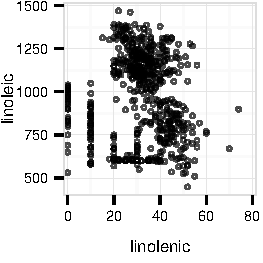
\includegraphics[width=1.75in]{images/linolenic-linoleic.pdf}
	  \caption{User-selected bivariate relationship of two chemicals in the Olive oils dataset. }
	 \label{fig:vrich_all}
\end{figure}

\begin{figure}
	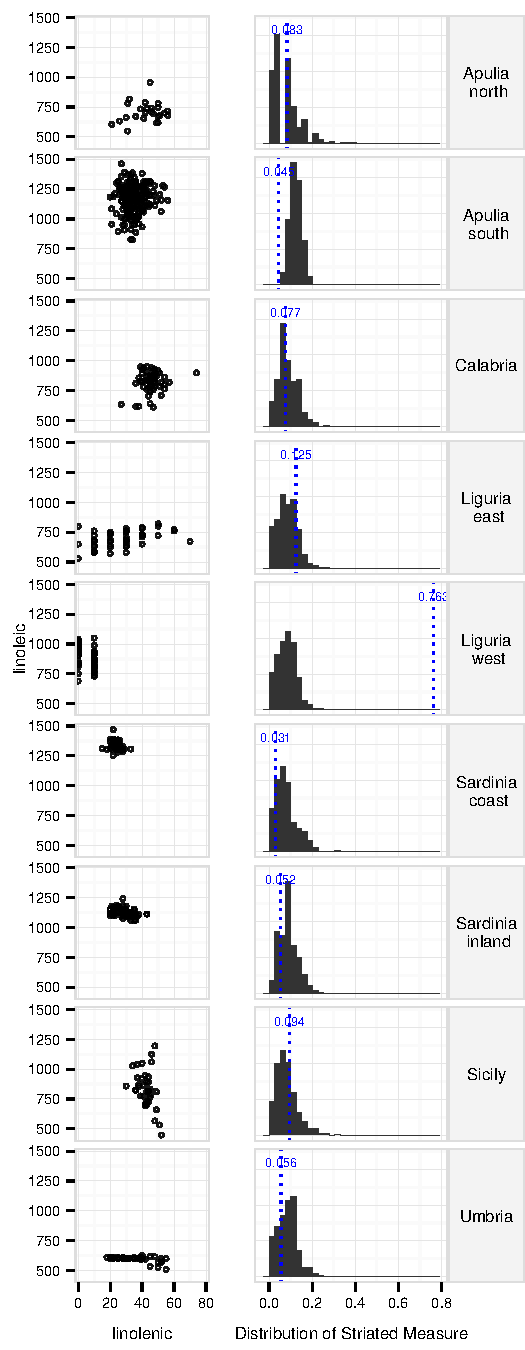
\includegraphics[width=3.25in]{images/15_729035813077-region.pdf}
	  \caption{The highest ranked small multiple on the Striation scagnostic pulls apart the striated patterns from the original bivariate relationship. }
	 \label{fig:vrich_sm}
\end{figure}

To do so, the analyst can use our approach with the ``Striation'' scagnostic~\cite{Wilkinson2005} which detects banding of points in a scatterplot. With this cognostic, our approach ranks the ``Region" variable as the best partitioning variable for isolating striated patterns from the $p$ variables in the data set. This is the partitioning shown in the left half of Figure~\ref{fig:vrich_sm}, which reveals the clean isolation of the striation pattern for olive oils from the Liguria region and the distinctive measurement structure of linoleic values for the Umbria region.

As before, the right side of Figure~\ref{fig:vrich_sm} shows the true ``Striation'' scores for this partitioning in blue and the randomized permutation scores in the black histogram. We can see that our algorithm has identified the striated pattern in Liguria west as being very unlikely to have arisen due to chance. The similar pattern in Liguria east is not picked up by our approach due to an issue with the underlying ``Striation'' scagnostic. We revisit this issue in Section~\ref{}.

\subsection{Informative}
Our second criterion is that we want small multiple displays that reveal informative structures when compared to the original view. This criterion is incorporated in our algorithm by the comparison between the true cognostic score and that of the randomized permutations. Randomly permuting the partitioning variable results in partitions that are random subsets of the data in the original plot. Visual patterns in this random subset are likely to be similar to those in the original plot, and thus, not informative. In contrast, a high absolute z-score for the true cognostic value is associated with a small multiple plot that shows a pattern \emph{different} from the original plot.

\begin{figure}
 \centering 
	 \begin{subfigure}{1.5in}
		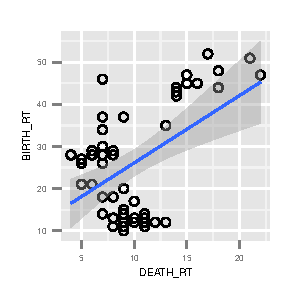
\includegraphics[width=1.5in]{images/DEATH_RT-BIRTH_RT.pdf}
		  \caption{}
		 \label{fig:informative_all}
	\end{subfigure}
	\begin{subfigure}{3in}
		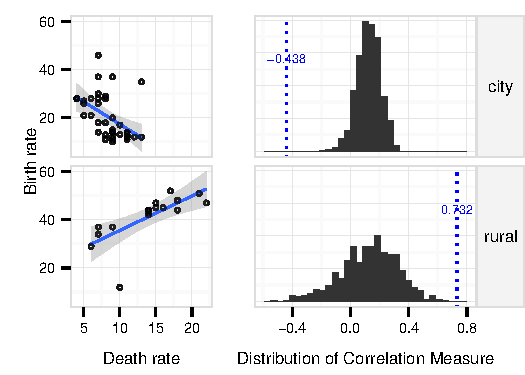
\includegraphics[width=3in]{images/7_05653068514253-URBAN.pdf}
		 \label{fig:informative}
		  \caption{}
	 \end{subfigure}
	\begin{subfigure}{3in}
		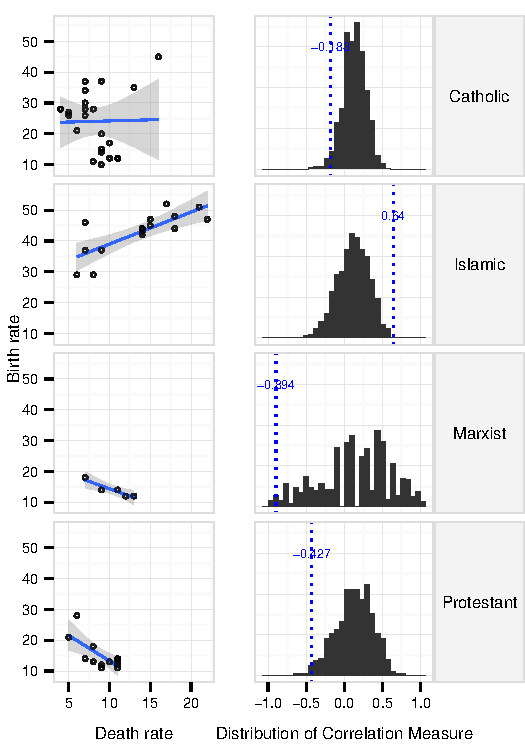
\includegraphics[width=3in]{images/2_56911395752061-LEADER.pdf}
		  \caption{}
		 \label{fig:informative_sm_big}
	 \end{subfigure}
	  \caption{(a) User-selected relationship between birth and death rates for countries around the world. (b) The highest ranked small multiple display shows partitions that reveal strong opposite trends that were not seen in the original view. (c) The lowest ranked small multiple display that reveals interesting correlations but is not parsimonious.}
\end{figure}

(NOTE: the following text says Monotonic, but the figures saying Correlation? Also, like before, we need an explanation of why it makes sense to use Monotonic/Correlation in this case.)

An illustration of this behavior involves the use of the Monotonic scagnostic~\cite{Wilkinson2005} and the Ourworld dataset of UN statistics on world countries~\cite{Wilkinson2005GG}. We want to determine how to partition the scatterplot between birth rate and death rate seen in Figure~\ref{fig:informative_all}. The highest ranked small multiple is that determined by the variable ``Urban" that partitions the data into two categories---``city" with $40$ points and ``rural" with $17$ points as seen in Figure~\ref{fig:informative}. This partitioning reveals that ``Urban" is a confounding covariate. While the main view shows a positive correlation between the birth and death rates, the small multiple view shows that in ``city" regions there is actually a strong negative correlation. As shown by the histograms on the right, this informative display arises because the patterns in the small multiple display are substantially different from the patterns we would see in random subsets of the original plot.

%The negative correlation is contrary to the pattern in the original view. As such it is an example of Simpson's paradox when aggregate patterns are affected by changes in the relative size and value of the subpopulations. 

(NOTE: it's not clear what the purpose of this paragraph and figure are. What argument are we making here? I'd expect to see a lower ranked partitioning where the patterns are all similar to the original plot and being able to say ``See this low ranked one clearly isn't very Informative.")
Figure~\ref{fig:informative_sm_big} is another informative small multiple display determined by the religion of the leader of the countries. However, this variable has more partitions and weaker patterns as each component plot has lower support. 


\subsection{Support}
Our third criterion for good small multiple displays is that they have patterns that are well-supported by the data. This property is incorporated into our approach through the use of the z-score normalization which adjusts for the variability in the ``null distributions" of the randomized cognostic scores. If the data set is small or there are outliers in the data set, this distribution will have high variance, which will downweight the resulting z-scores.

Consider the distributions shown in Figure~\ref{fig:informative_sm_big}, particularly the ``Marxist" partition with only five data points. Given the width of the distribution, it is far less likely that a particular true score computed on a component plot will be significantly different from the mean, making it less likely that the particular small multiple would be ranked high.
\begin{figure}
\centering
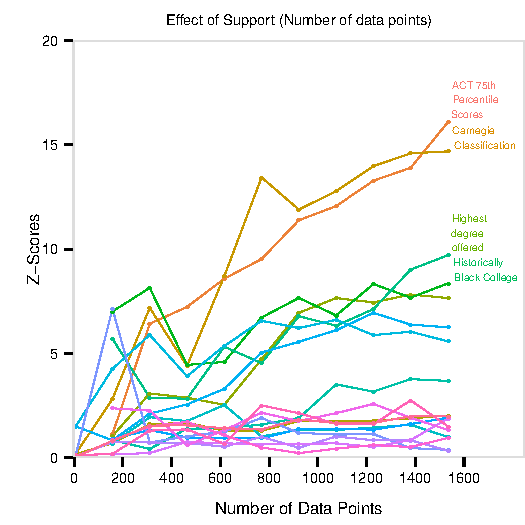
\includegraphics[width=3.25in,height=3.25in]{images/support-nogrid.pdf}
  \caption{The effect of support on the combined z-scores ranking of partitioning variables for the data about US universities. As the number of points in the dataset increase, the importance of the variable determined by the z-scores increases too. }
 \label{fig:support}
\end{figure}

To examine how our algorithm behaves with different amounts of support, we experiment by varying the size of the input data set. Using the US university data set discussed in the introduction, we compute the z-scores for all the partitioning variables in the dataset. Figure~\ref{fig:support} shows these rankings for different data set sizes, generated by randomly subsetting the full data set.
As can be seen, for small data sets, the scores are small and, except for ACT scores, there is no clear ranking. As the data set grows, we become more confident in the rankings with ``Historically Black College'' and ``Carnegie Classification'' separating from the other variables. The patterns in these small multiple displays are weaker and we correctly require more data to be confident in their ranking.

(NOTE: it would be great to show the Historically Black College and Carnegie Classification small multiples to really sell this story.) 

(NOTE: what measure are we using in this example?)


\subsection{Parsimonious}
  \begin{figure}
    \centering
    \begin{minipage}[b]{1.7in}
       \begin{subfigure}[b]{\linewidth}
  	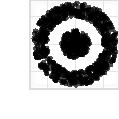
\includegraphics[width=0.75in]{images/donut1-donut2.pdf}
      \caption{}
      \label{fig:pars1}
      \end{subfigure}\\[\baselineskip]
      \begin{subfigure}[b]{\linewidth}
  	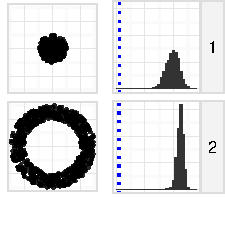
\includegraphics[width=1.65in]{images/19_5065416601259-cluster.pdf}
      \caption{}
      \label{fig:pars2}
      \end{subfigure}
      \begin{subfigure}[b]{\linewidth}
  	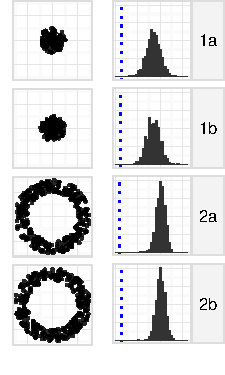
\includegraphics[width=1.65in]{images/9_27395081160431-cluster1.pdf}
        \caption{}
      \label{fig:pars3}        
      \end{subfigure}
    \end{minipage}
    \begin{subfigure}[b]{1.7in}
	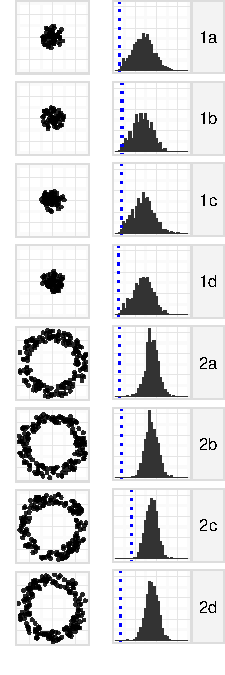
\includegraphics[width=1.7in]{images/5_12851615653375-cluster2.pdf}
      \caption{}
      \label{fig:pars4}
    \end{subfigure}
    \caption{The ranking of small multiple displays respects the parsimony criterion. (a) The original bullseye pattern. (b) The best small multiple determined by the Clumpy scagnostic. (c) The second best partitioning variable redundantly halves the two partitions from (b). (d) The lowest ranked small multiple display with eight partitions.}
    \label{fig:parsimonious}
  \end{figure}

Our final criteria is parsimony. This criteria is indirectly included in our approach. High-cardinality variables create a large number of partitions, which are likely to have low support as the observations get distributed among more partitions. Thus, we will tend to reject such partitionings if less parsimonious options are available.
 
We illustrate this behavior using an artificially generated dataset so we can hold the visual patterns across partitioning variables equal as far as possible. The input visualization is the bullseye pattern shown in Figure~\ref{fig:pars1}. This artificial data set includes a partitioning variable that cleanly separates the ring from the core as seen in Figure~\ref{fig:pars2}. It also includes two other partitioning variables that also separate the ring and core, but they also further split them into two and four random partitions (Figures~\ref{fig:pars3} and~\ref{fig:pars4}). The separation between the core and ring are equally visible in all three variants, however the first is the most parsimonious---it shows the pattern with the least amount of extraneous information. 
The Clumpy scagnostic has high values for plots with multiple tight clumps of points such as the original bullseye pattern but low values for plots with just one clump such as those with just the core or just the ring. So random samples of the bullseye pattern will produce a distribution of Clumpy scores that are high but the partitioning variables that split out the core and ring will have Clumpy scores that are much lower.

In the histograms, we can see that the width of the distributions increases as the number of partitions increases. Thus, the computed z-score will be highest for the first partitioning variable. The actual values are $19.507$, $9.274$ and $5.129$. Thus, our approach does prefer more parsimonious partitioning variables.

